\documentclass[12pt]{article}
\usepackage{graphicx}
\usepackage{caption}
\usepackage{subcaption}
\usepackage{hyperref}
\usepackage{listings}
\usepackage{xcolor}
\hypersetup{
    colorlinks,
    linkcolor={blue!50!black},
}

\title{CAVA-TEMA1}
\author{Huțan Mihai-Alexandru Gr.343}
\date{November 2023}

\begin{document}

    \maketitle


    \tableofcontents


    \section{Introduction}\label{sec:introduction}

    \paragraph{This homework comes down to only three steps, \hyperref[sec:detection]{detection}, \hyperref[sec:classification]{classification} and \hyperref[sec:score-calculation]{score calculation}, all these steps are explained in depth in the following sections.}


    \section{Detection}\label{sec:detection}

    \subsection{Board Extraction}\label{subsec:board-extraction}

    \subsubsection{Approach}

    \paragraph{For detection part we can see two major steps that we need to do before continuing solving the problem. We have a lot of unnecessary data, the table that the board is placed on, and the score board.}

    \paragraph{The score board is unnecessary because in the test image the players are not moved anymore, therefore we can not use that part of the board to calculate the score in \hyperref[sec:score-calculation]{section 4}.}

    \begin{figure}[!h]
        \centering
        \begin{subfigure}{.5\textwidth}
            \centering
            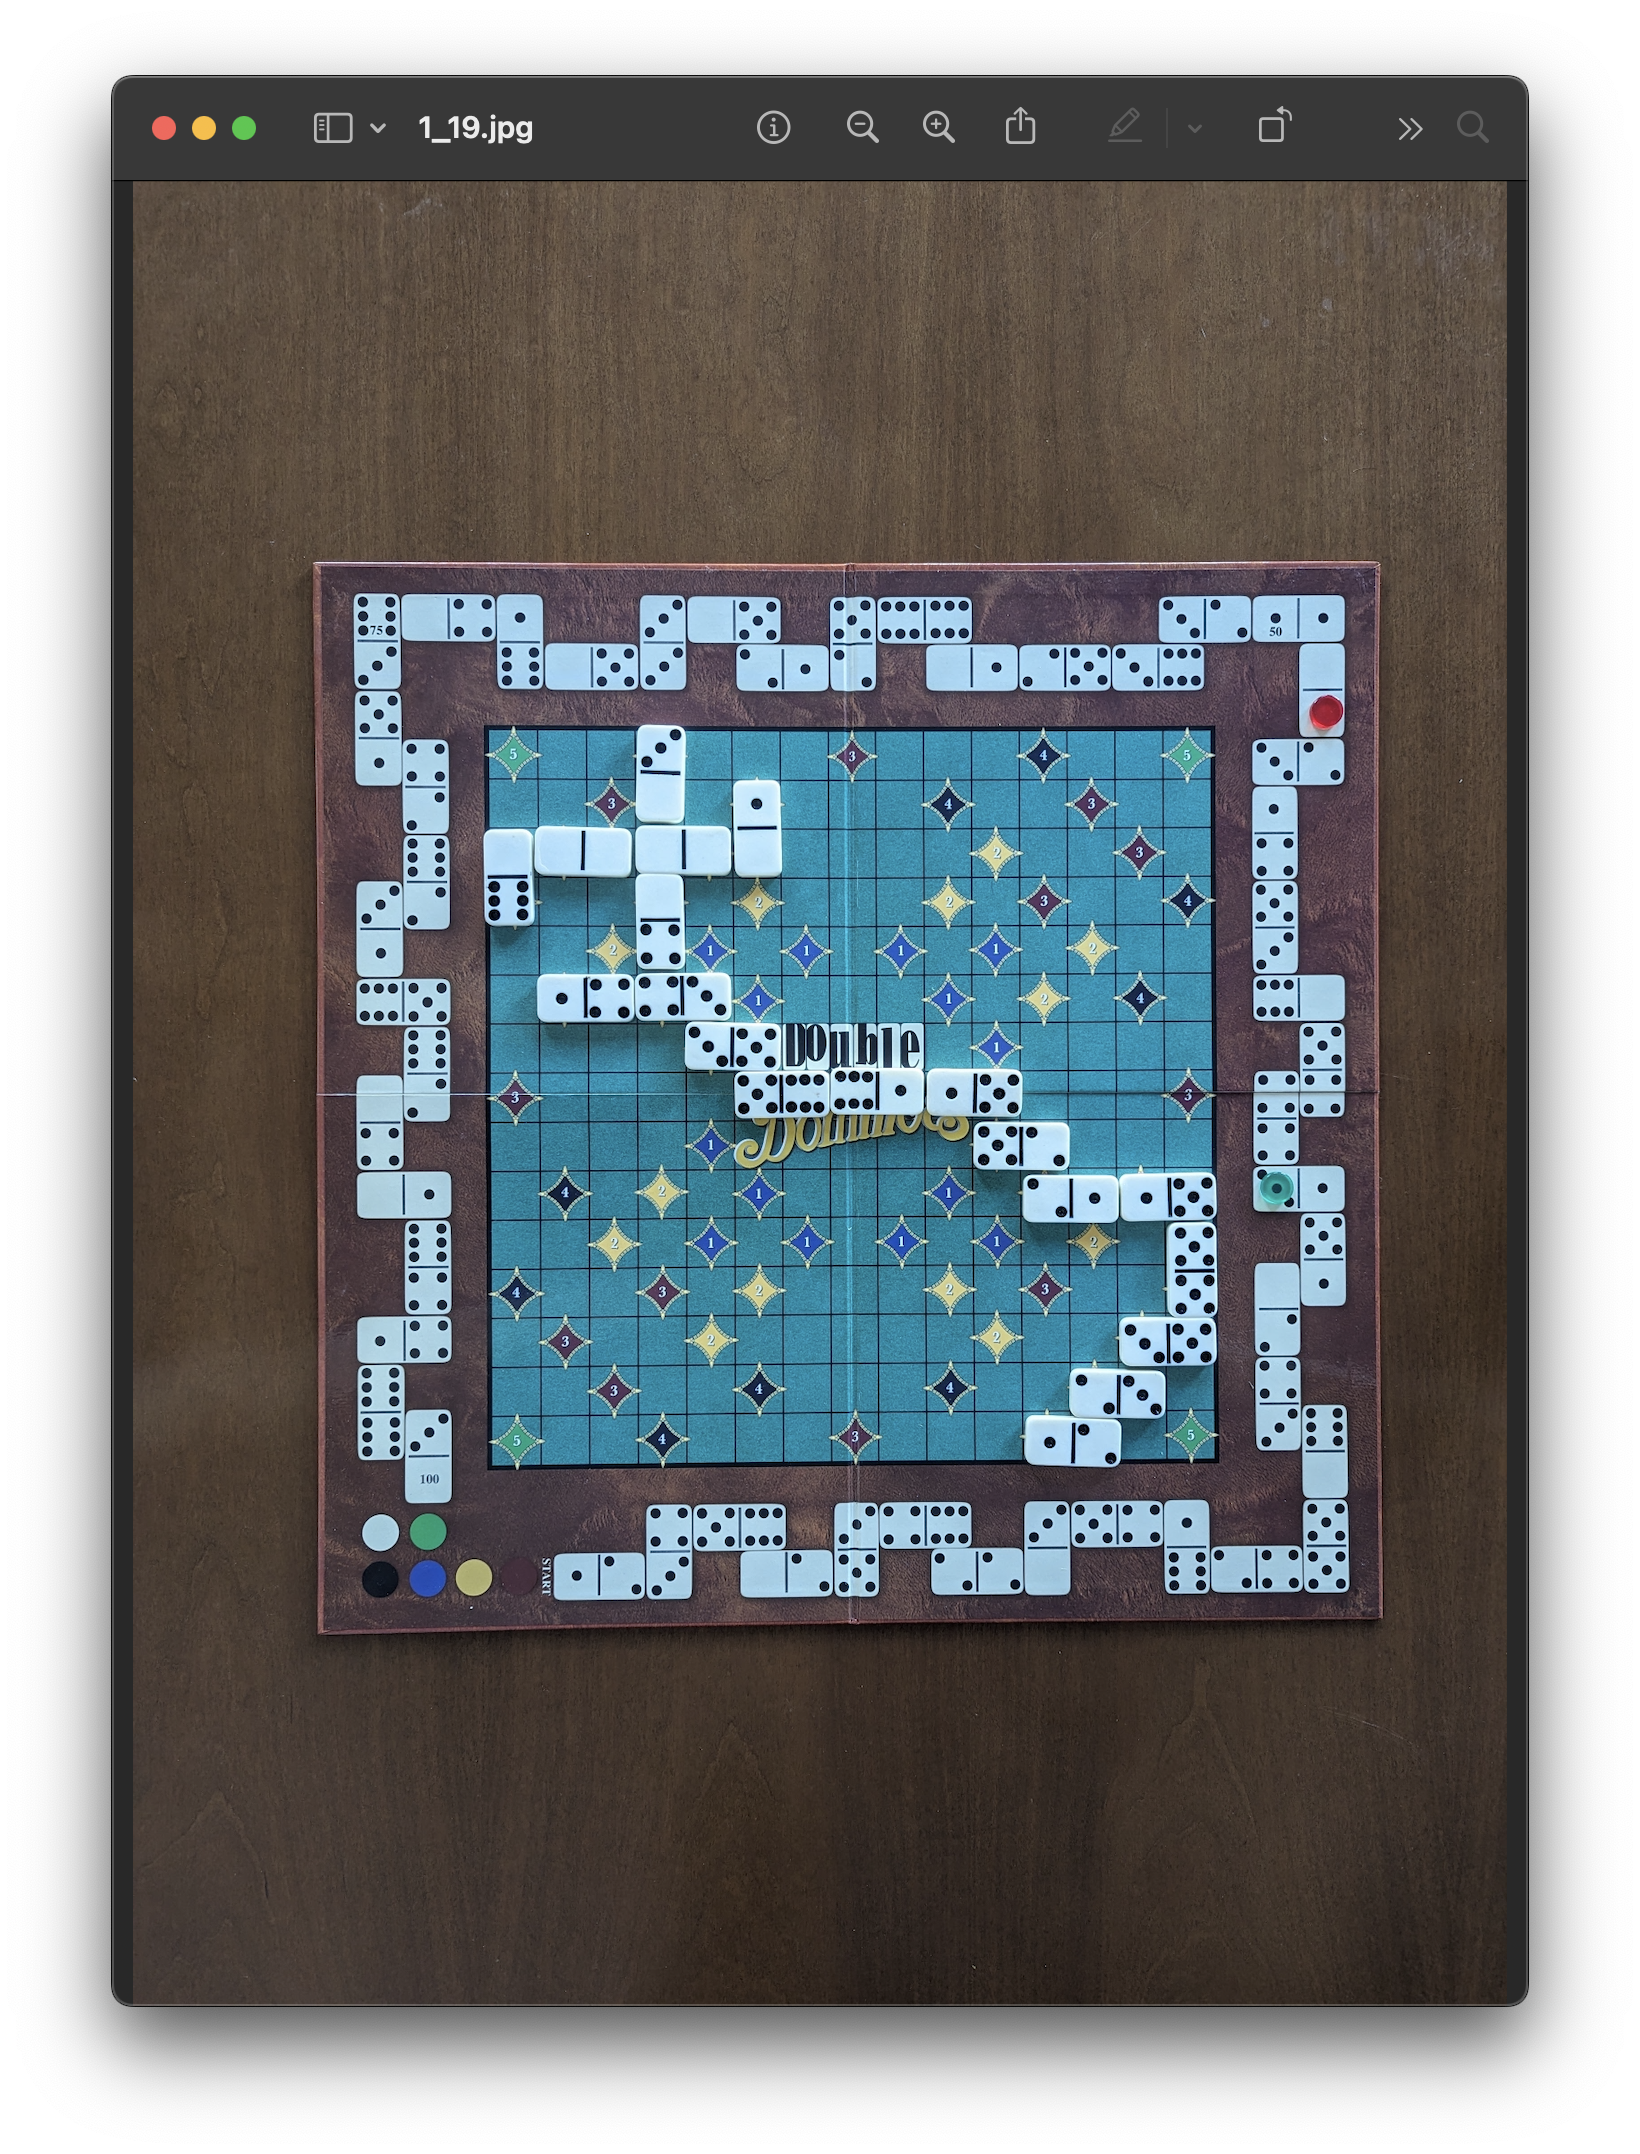
\includegraphics[width=\linewidth]{images/examples/train_example}
            \caption{Train Image}
            \label{fig:train_image}
        \end{subfigure}%
        \begin{subfigure}{.5\textwidth}
            \centering
            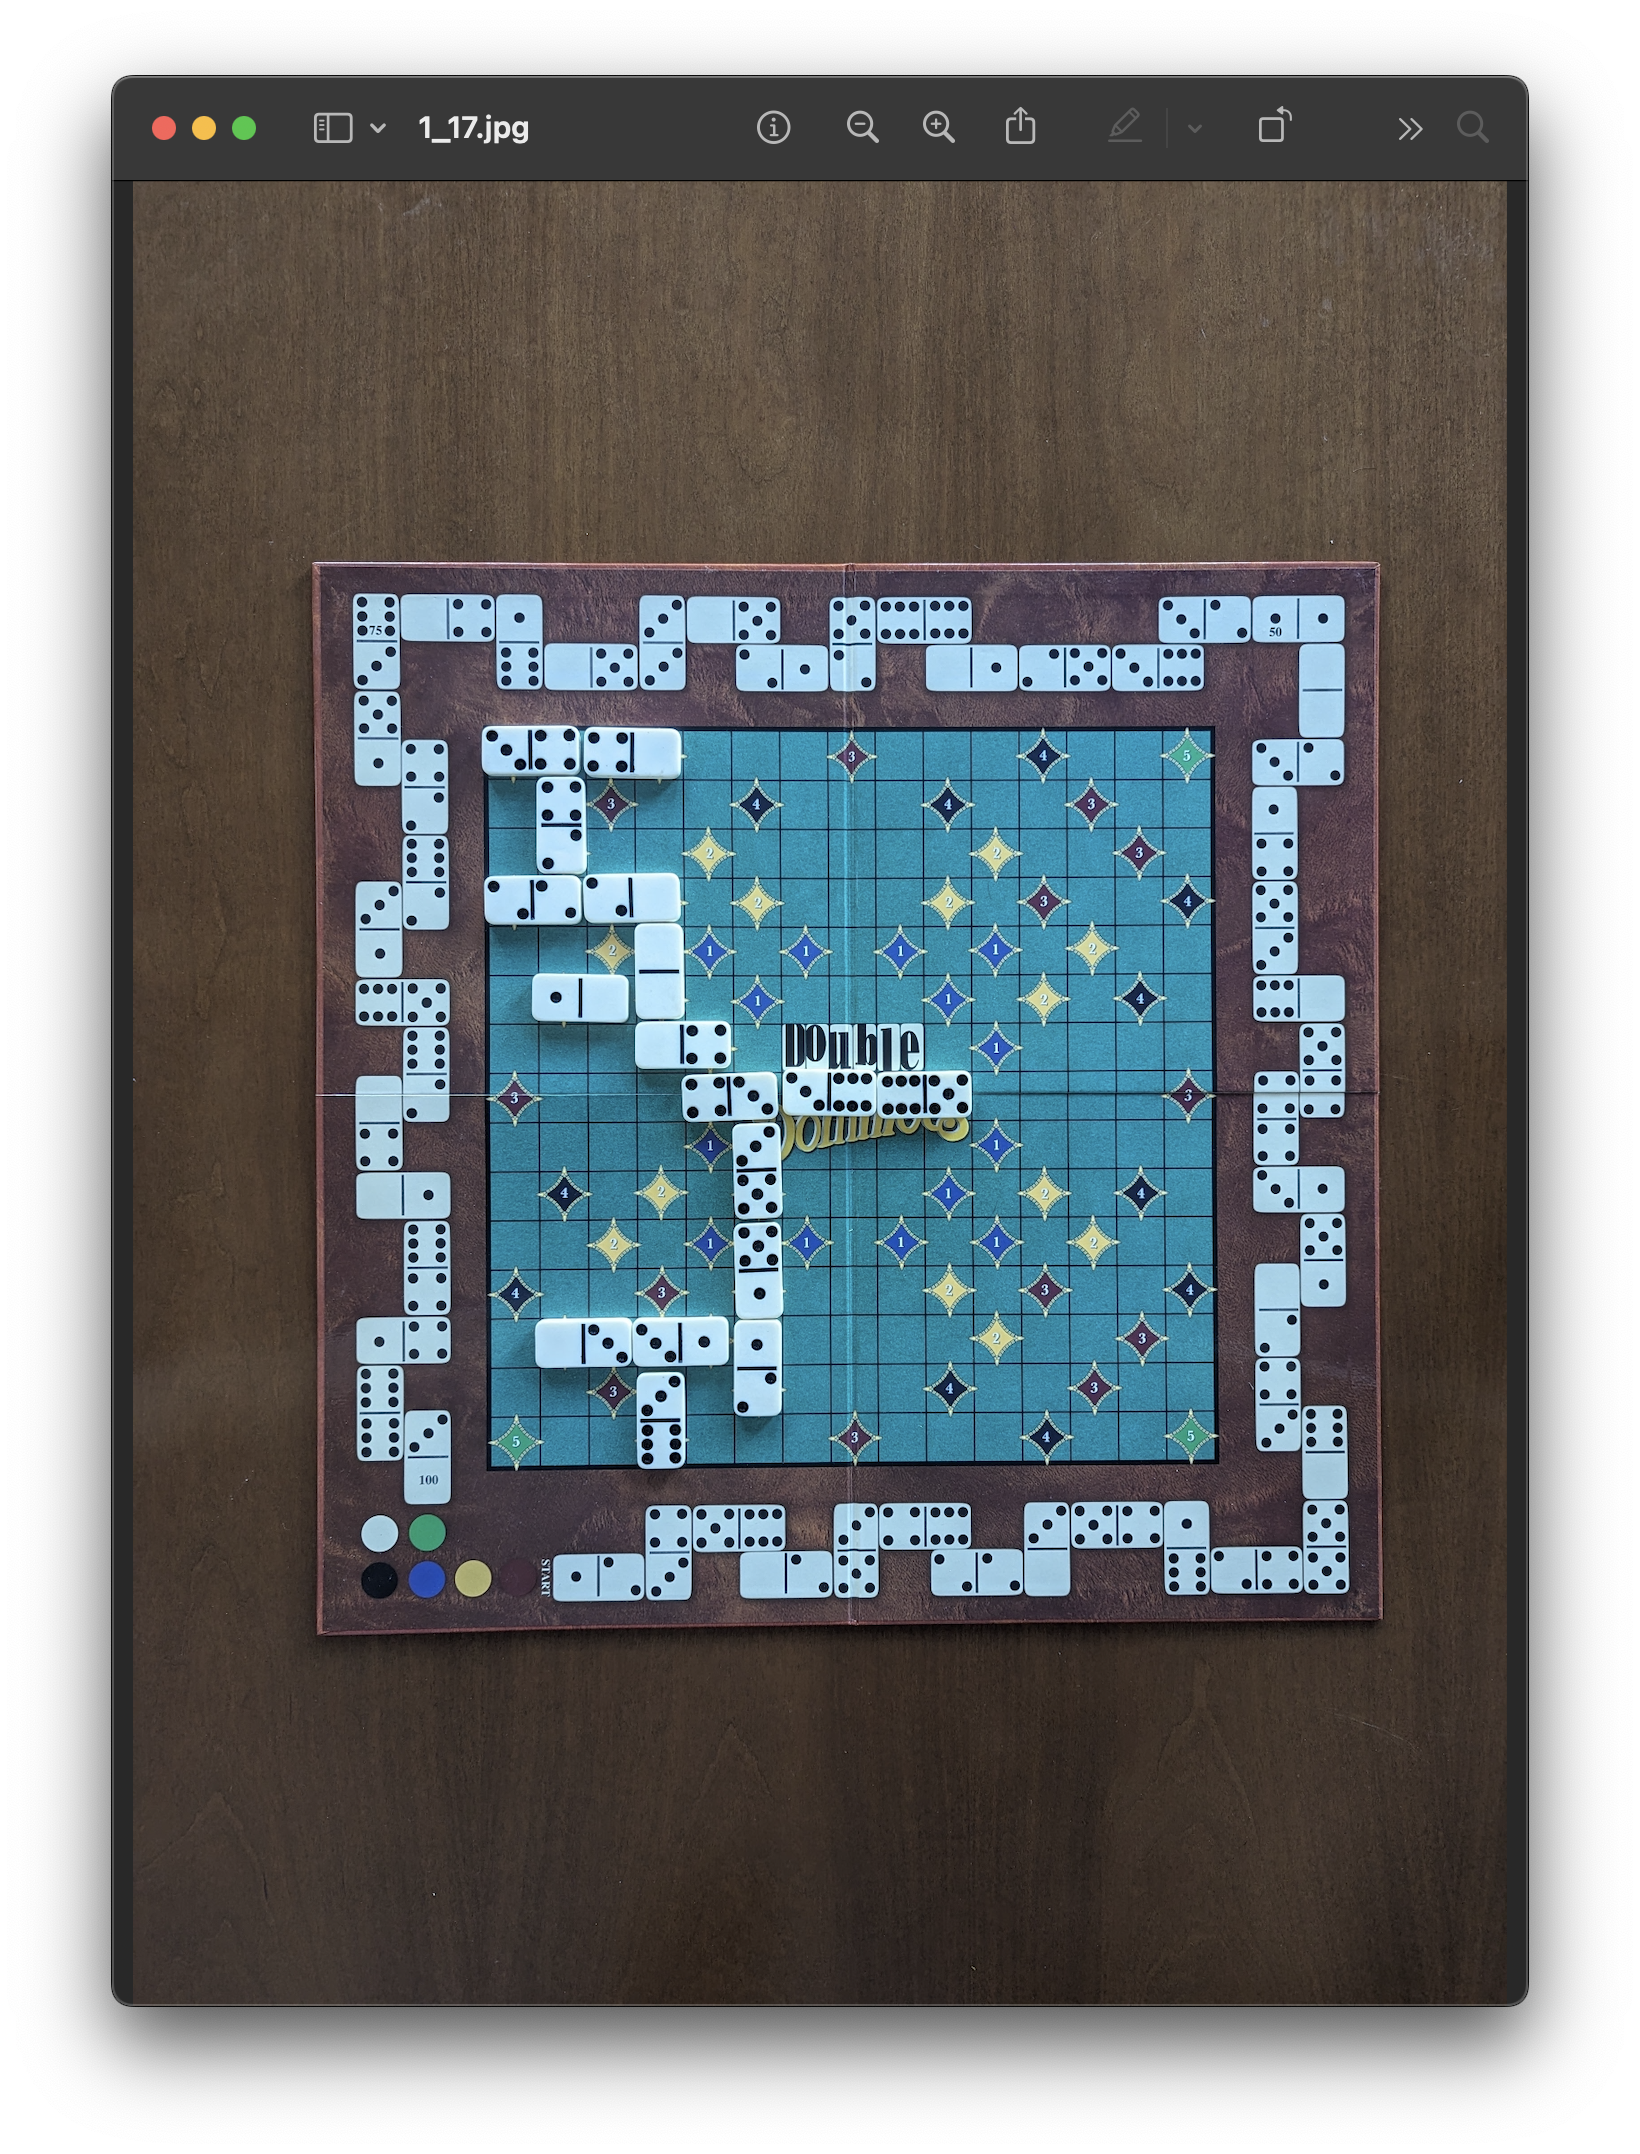
\includegraphics[width=\linewidth]{images/examples/test_example}
            \caption{Test Image}
            \label{fig:test_image}
        \end{subfigure}
        \caption{Examples}
        \label{fig:examples}
    \end{figure}

    \subsubsection{Steps}

    \paragraph{All parameters values presented in the following steps were found by trial and error, and visualization logic while debugging.}

    \paragraph{All these steps can be visualized in \hyperref[fig:board-extraction-steps]{Figure 2}.}
    \begin{itemize}
        \item HSV Mask
        \begin{itemize}
            \item For Board Extraction the main idea is to use an HSV mask to remove parts of the image that are not of interest.
            \item The HSV values found are (80, 0, 0) and (102, 255, 255).
            \begin{lstlisting}[language=Python, breaklines=true, breakatwhitespace=true, basicstyle=\small]
            LOWERB_BOARD = np.array([80, 0, 0])
            UPPERB_BOARD = np.array([102, 255, 255])
            \end{lstlisting}
        \end{itemize}
        \item Preprocessing
        \begin{itemize}
            \item In the image of the mask, there is quite a bit of noise. Therefore we reduce it using both median and gaussian blur to get a sharpened version of the original image.
            \begin{lstlisting}[language=Python, breaklines=true, breakatwhitespace=true, basicstyle=\small]
            image_m_blur = cv.medianBlur(mask, 5)
            image_g_blur = cv.GaussianBlur(image_m_blur, (3, 3), 5)
            image_sharpened = cv.addWeighted(image_m_blur, 1.5, image_g_blur, -0.8, 0)
            \end{lstlisting}
            \item We threshold the image intro a binary image.
            \begin{lstlisting}
            _, thresh = cv.threshold(image_sharpened, 151, 255, cv.THRESH_BINARY)
            \end{lstlisting}
            \item We use morphological operations to erode and then dilate the image.
            \begin{lstlisting}[language=Python, breaklines=true, breakatwhitespace=true, basicstyle=\small]
            kernel = np.ones((3, 3), np.uint8)
            thresh = cv.erode(thresh, kernel, iterations=4)
            thresh = cv.dilate(thresh, kernel, iterations=3)
            \end{lstlisting}
        \end{itemize}
        \item Edge Detection
        \begin{itemize}
            \item We use Canny for edge detection on the preprocessed image.
            \begin{lstlisting}[language=Python, breaklines=true, breakatwhitespace=true, basicstyle=\small]
            edges = cv.Canny(image, 200, 400, apertureSize=7)
            \end{lstlisting}
        \end{itemize}
        \item Contours
        \begin{itemize}
            \item We find the contours.
            \begin{lstlisting}[language=Python, breaklines=true, breakatwhitespace=true, basicstyle=\small]
            contours, _ = cv.findContours(edges, cv.RETR_EXTERNAL, cv.CHAIN_APPROX_SIMPLE)
            \end{lstlisting}
        \end{itemize}
        \item Find Extreme Points In Contours
        \begin{itemize}
            \item We use a function to find the topleft, topright, bottomleft, and bottomright points in the image.
        \end{itemize}
        \item Warp
        \begin{itemize}
            \item We use warpPerspective from opencv to get our board from the image and resize it to 1500x1500px, each box in the board being 100x100px.
            \begin{lstlisting}[language=Python, breaklines=true, breakatwhitespace=true, basicstyle=\small]
            width = BOARD_WIDTH * BOX_SIZE  # 15 * 100
            height = BOARD_HEIGHT * BOX_SIZE  # 15 * 100

            puzzle = np.array([top_left, top_right, bottom_right, bottom_left], dtype="float32")
            destination_of_puzzle = np.array([[0, 0], [width, 0], [width, height], [0, height]], dtype="float32")

            M = cv.getPerspectiveTransform(puzzle, destination_of_puzzle)

            result = cv.warpPerspective(image, M, (width, height))
            \end{lstlisting}
        \end{itemize}
    \end{itemize}

    \begin{figure}[!h]
        \centering
        \caption{Board Extraction Steps}
        \label{fig:board-extraction-steps}
        \begin{subfigure}{.5\textwidth}
            \centering
            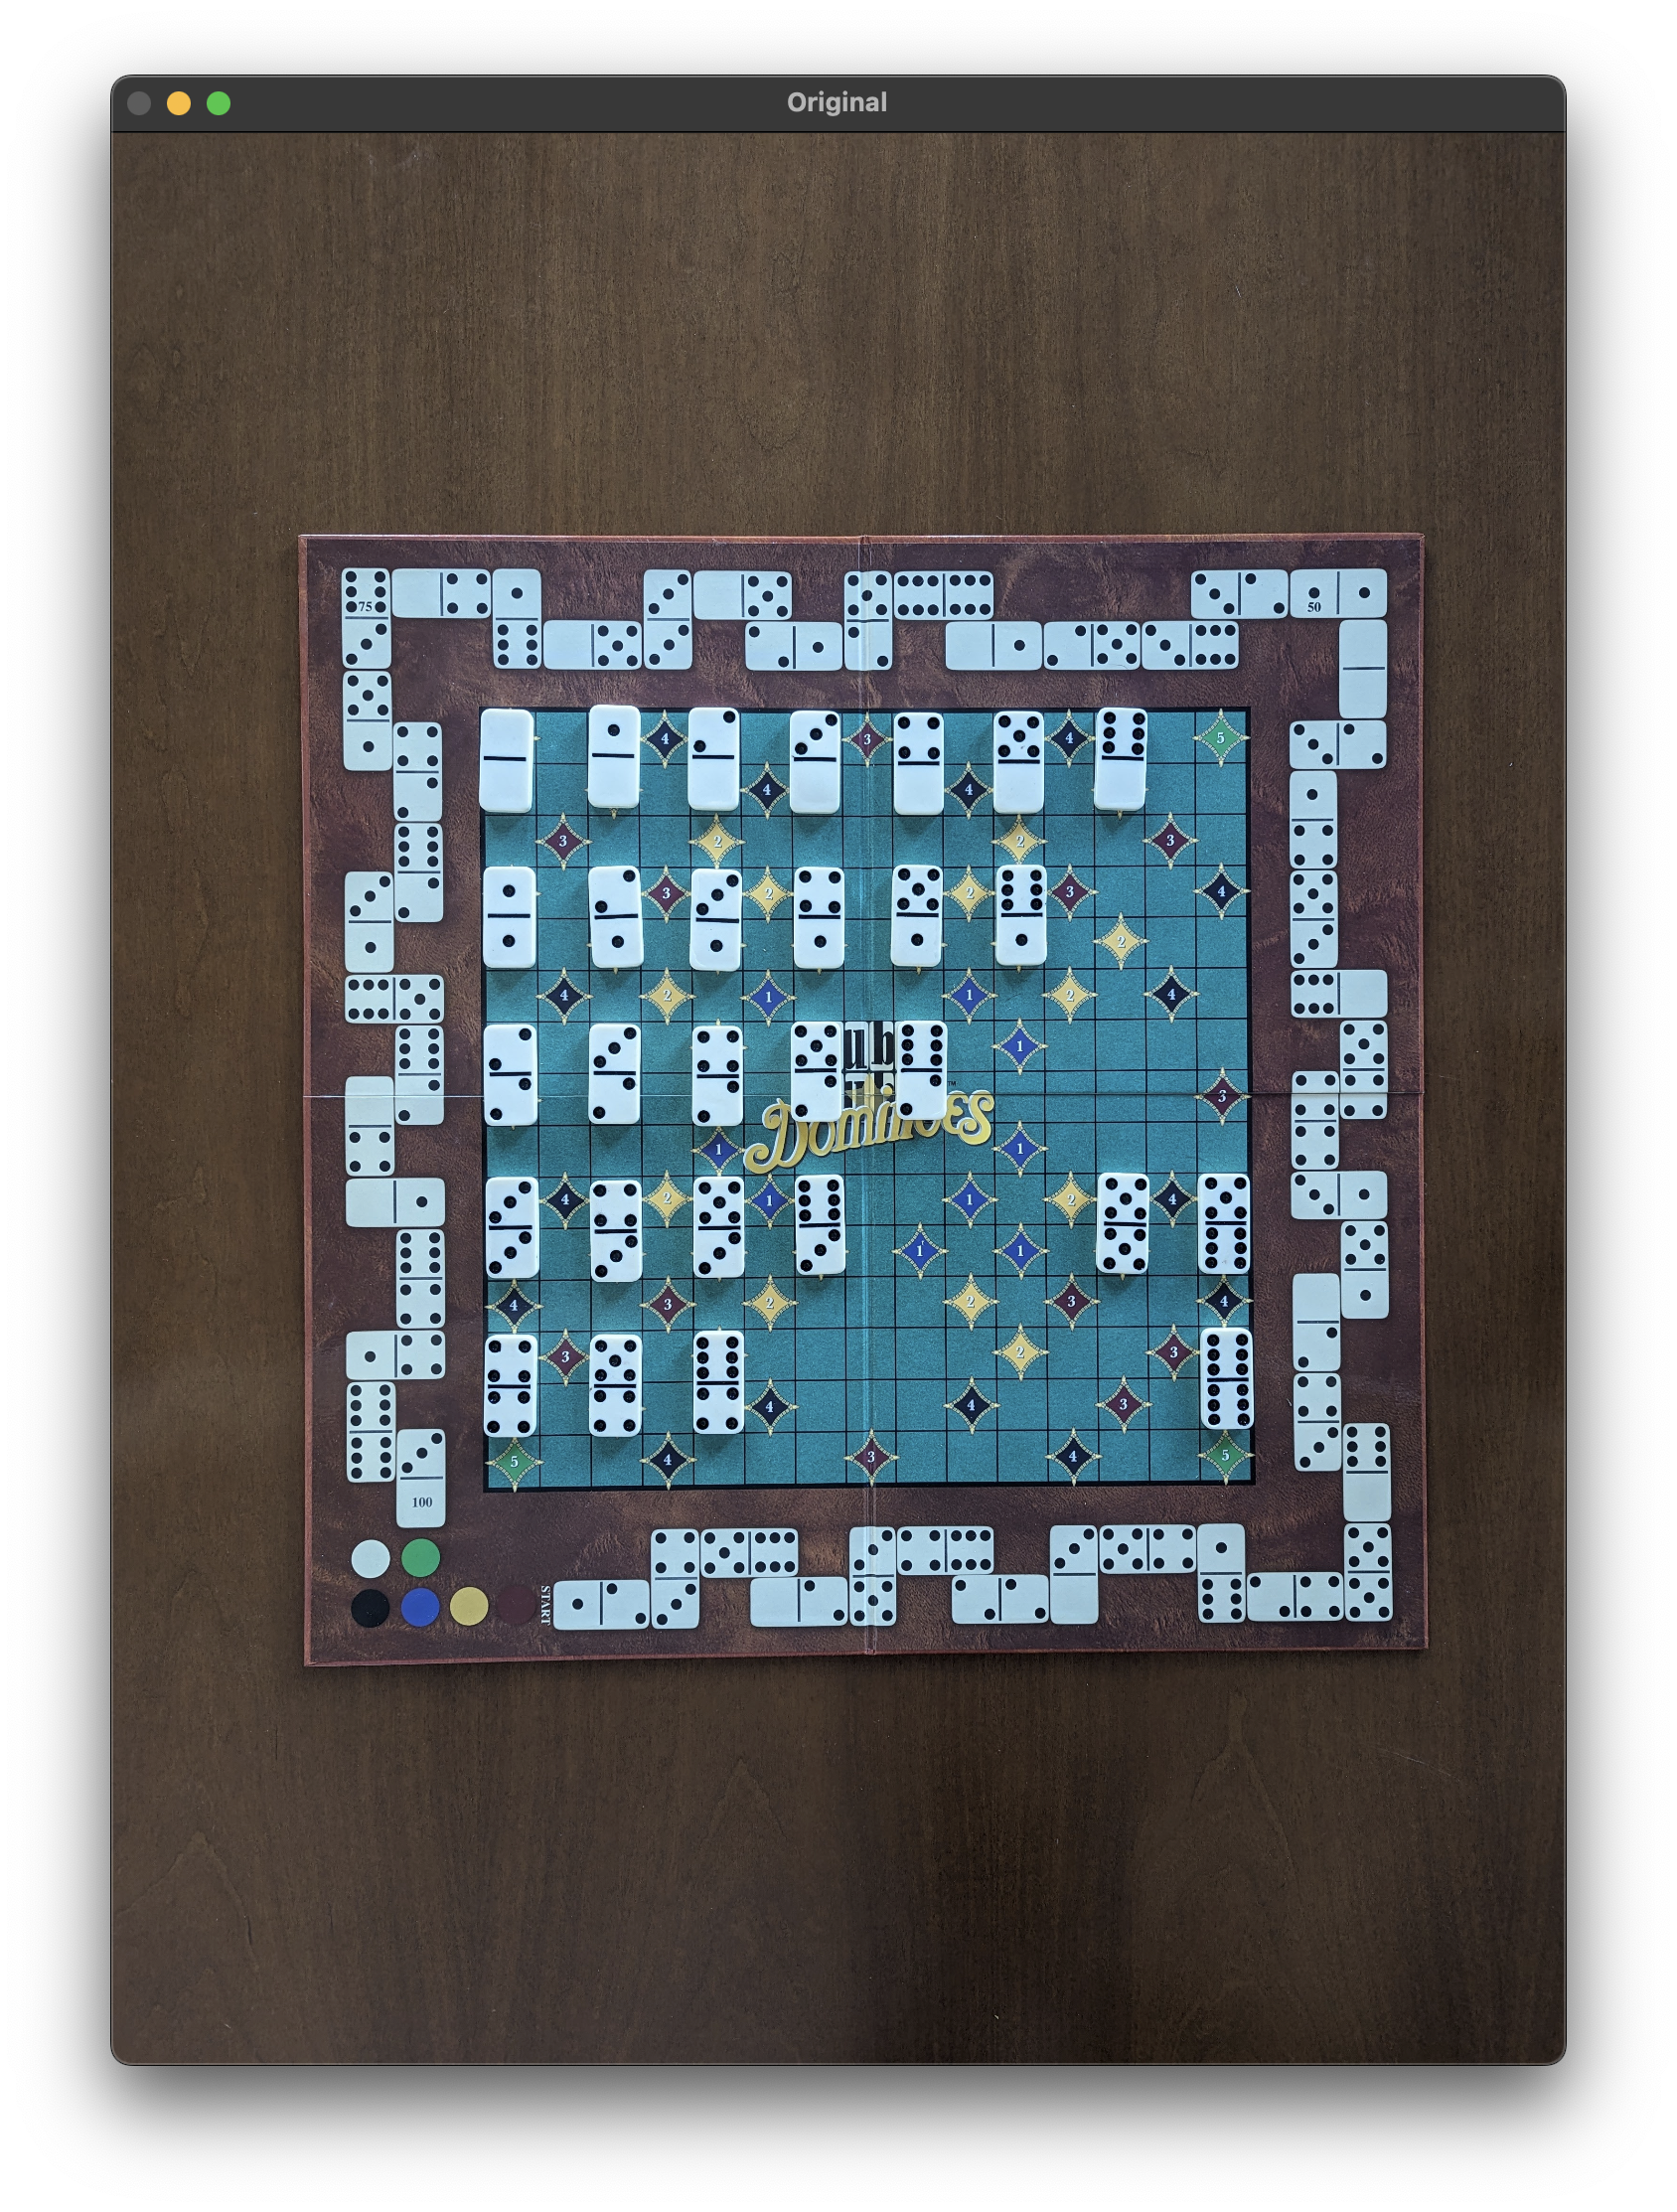
\includegraphics[width=0.8\linewidth]{images/board_extraction/original.png}
            \caption{Original Image}
            \label{fig:be-original}
        \end{subfigure}%
        \begin{subfigure}{.5\textwidth}
            \centering
            \includegraphics[width=0.8\linewidth]
            {images/board_extraction/mask.png}
            \caption{HSV Mask}
            \label{fig:be-mask}
        \end{subfigure}
    \end{figure}
    \begin{figure}[!h]
        \ContinuedFloat
        \centering
        \begin{subfigure}{.5\textwidth}
            \centering
            \includegraphics[width=0.9\linewidth]{images/board_extraction/sharpened.png}
            \caption{Sharpened}
            \label{fig:be-sharpened}
        \end{subfigure}%
        \begin{subfigure}{.5\textwidth}
            \centering
            \includegraphics[width=0.9\linewidth]
            {images/board_extraction/threshold.png}
            \caption{Threshold}
            \label{fig:be-threshold}
        \end{subfigure}
    \end{figure}
    \begin{figure}[!h]
        \ContinuedFloat
        \centering
        \begin{subfigure}{.5\textwidth}
            \centering
            \includegraphics[width=0.9\linewidth]{images/board_extraction/eroded.png}
            \caption{Eroded}
            \label{fig:be-eroded}
        \end{subfigure}%
        \begin{subfigure}{.5\textwidth}
            \centering
            \includegraphics[width=0.9\linewidth]
            {images/board_extraction/dilated.png}
            \caption{Dilated}
            \label{fig:be-dilated}
        \end{subfigure}
    \end{figure}
    \begin{figure}[!h]
        \ContinuedFloat
        \centering
        \begin{subfigure}{.5\textwidth}
            \centering
            \includegraphics[width=0.9\linewidth]{images/board_extraction/edges.png}
            \caption{Canny Edges}
            \label{fig:be-edges}
        \end{subfigure}%
        \begin{subfigure}{.5\textwidth}
            \centering
            \includegraphics[width=0.9\linewidth]
            {images/board_extraction/contours.png}
            \caption{Contours}
            \label{fig:be-contours}
        \end{subfigure}
    \end{figure}
    \begin{figure}[!h]
        \ContinuedFloat
        \centering
        \begin{subfigure}{.5\textwidth}
            \centering
            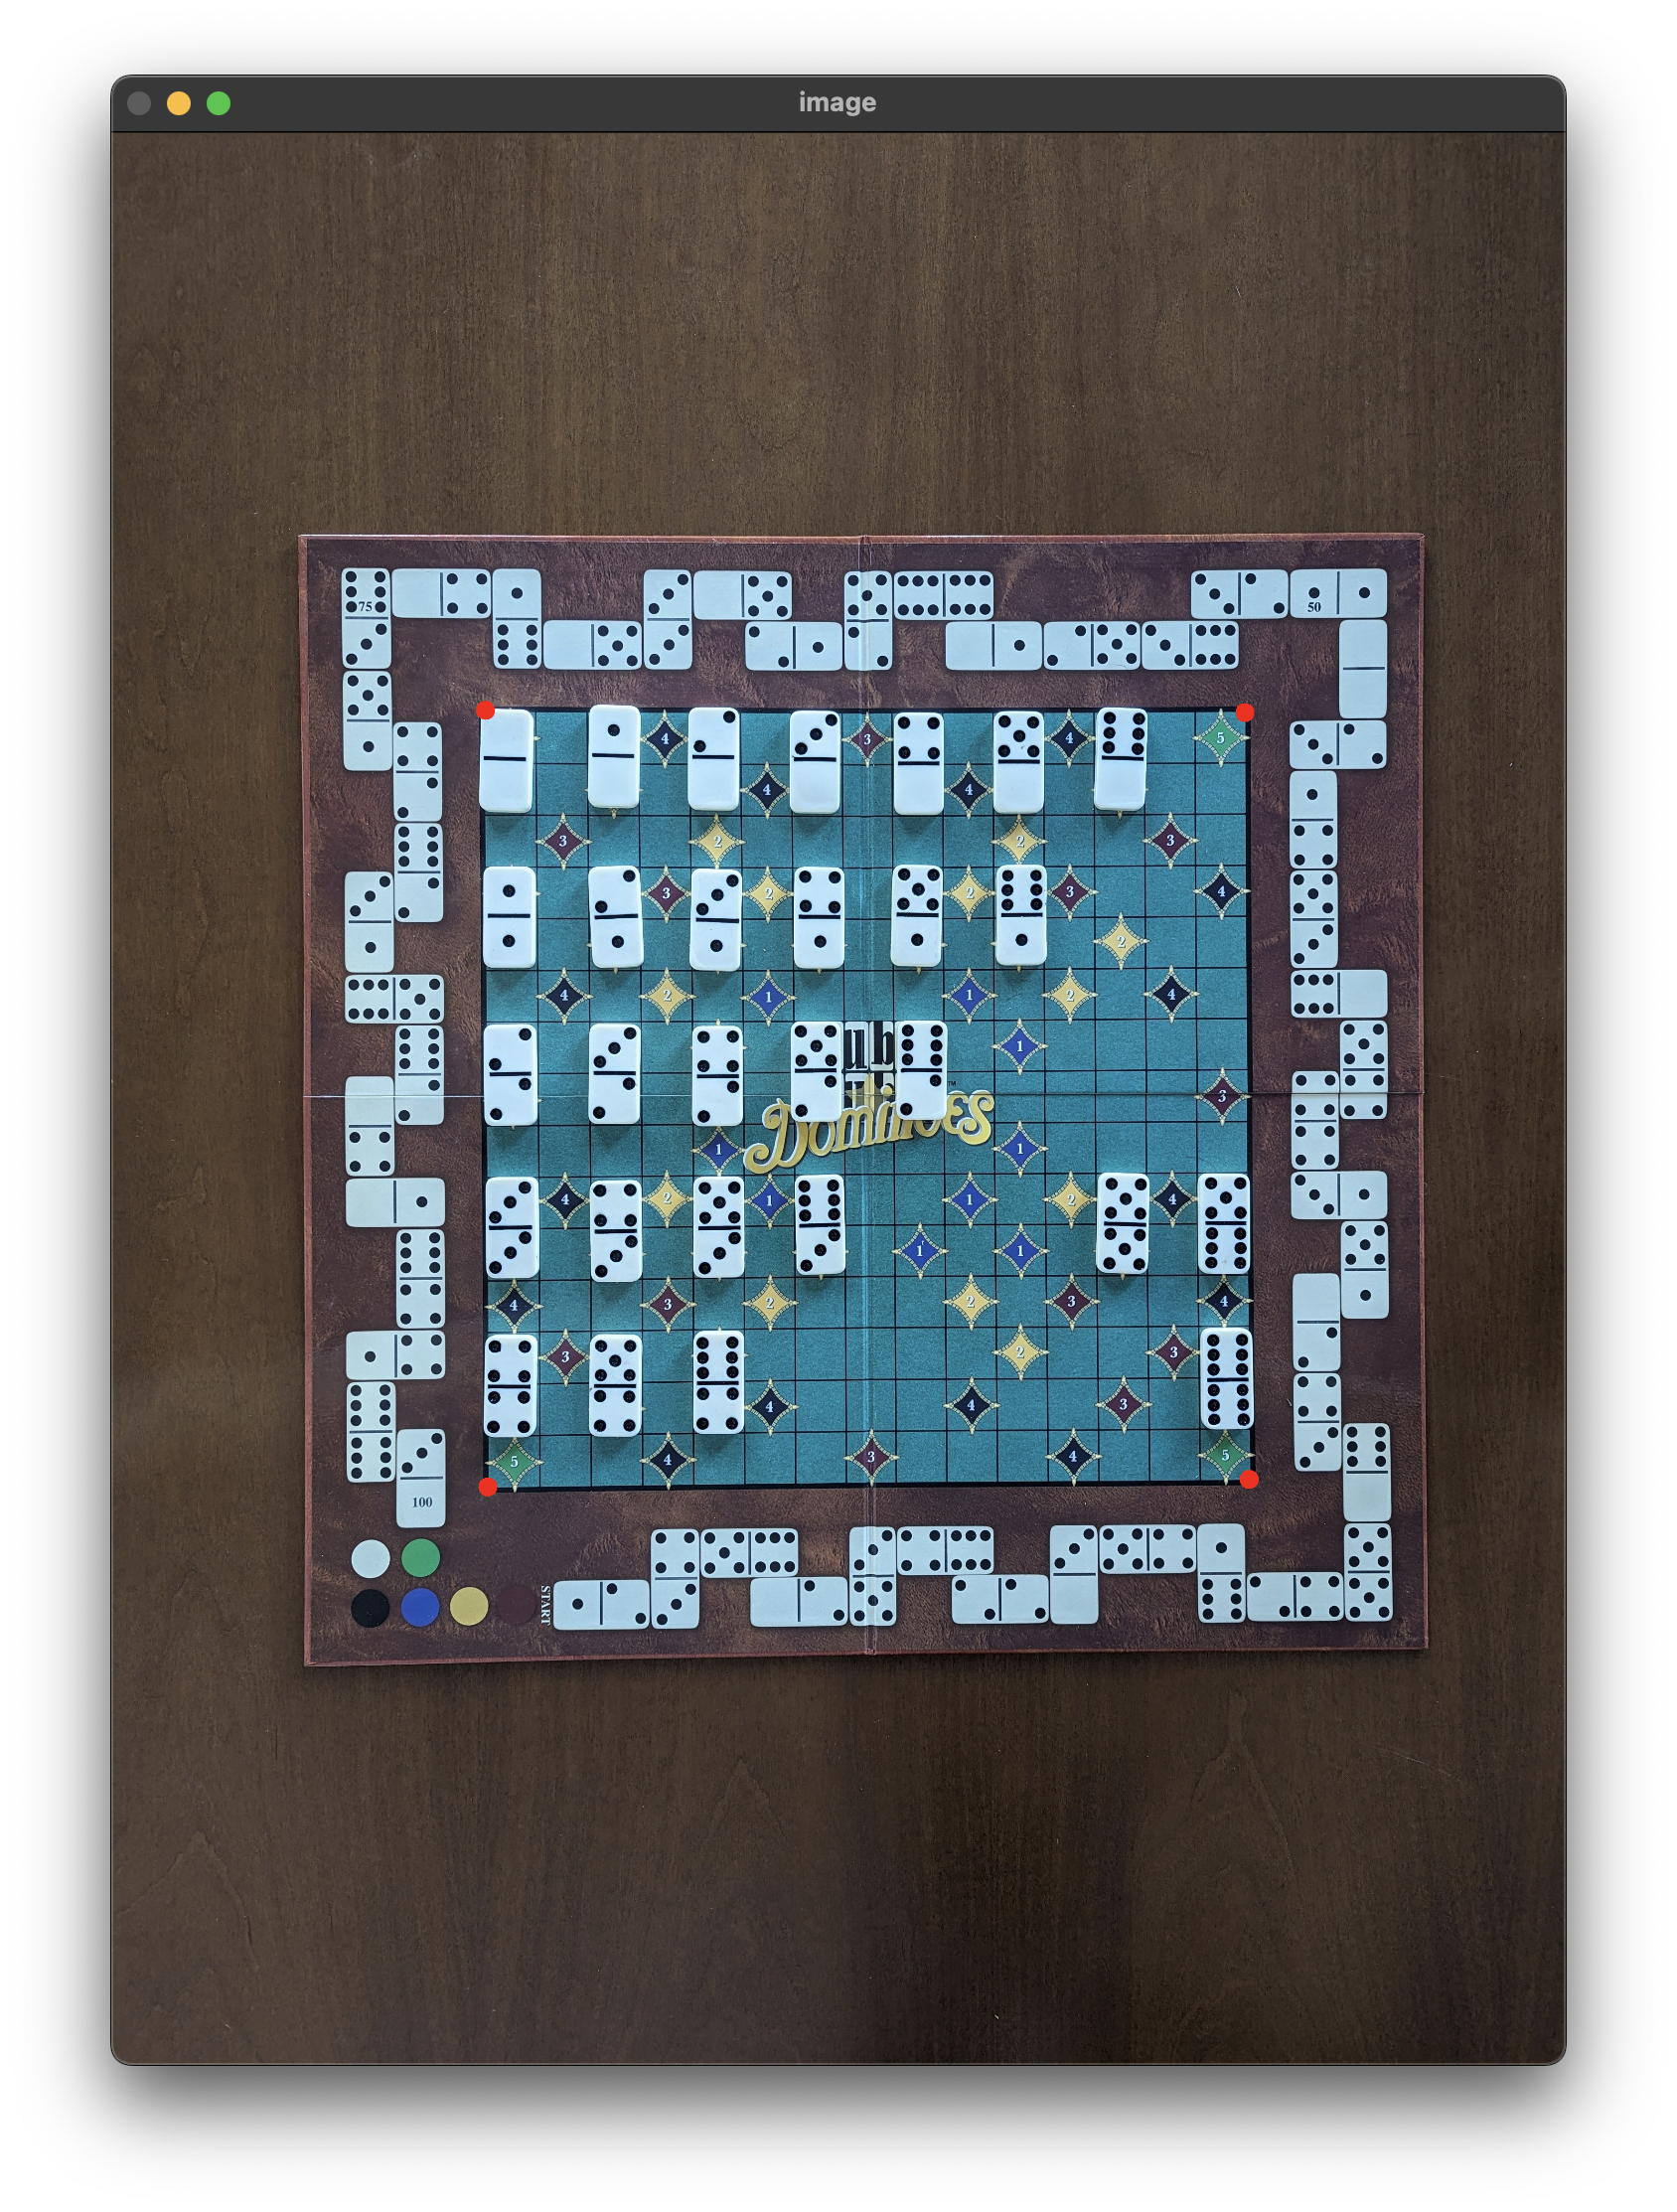
\includegraphics[width=0.9\linewidth]{images/board_extraction/points.png}
            \caption{Extreme Points}
            \label{fig:be-points}
        \end{subfigure}%
        \begin{subfigure}{.5\textwidth}
            \centering
            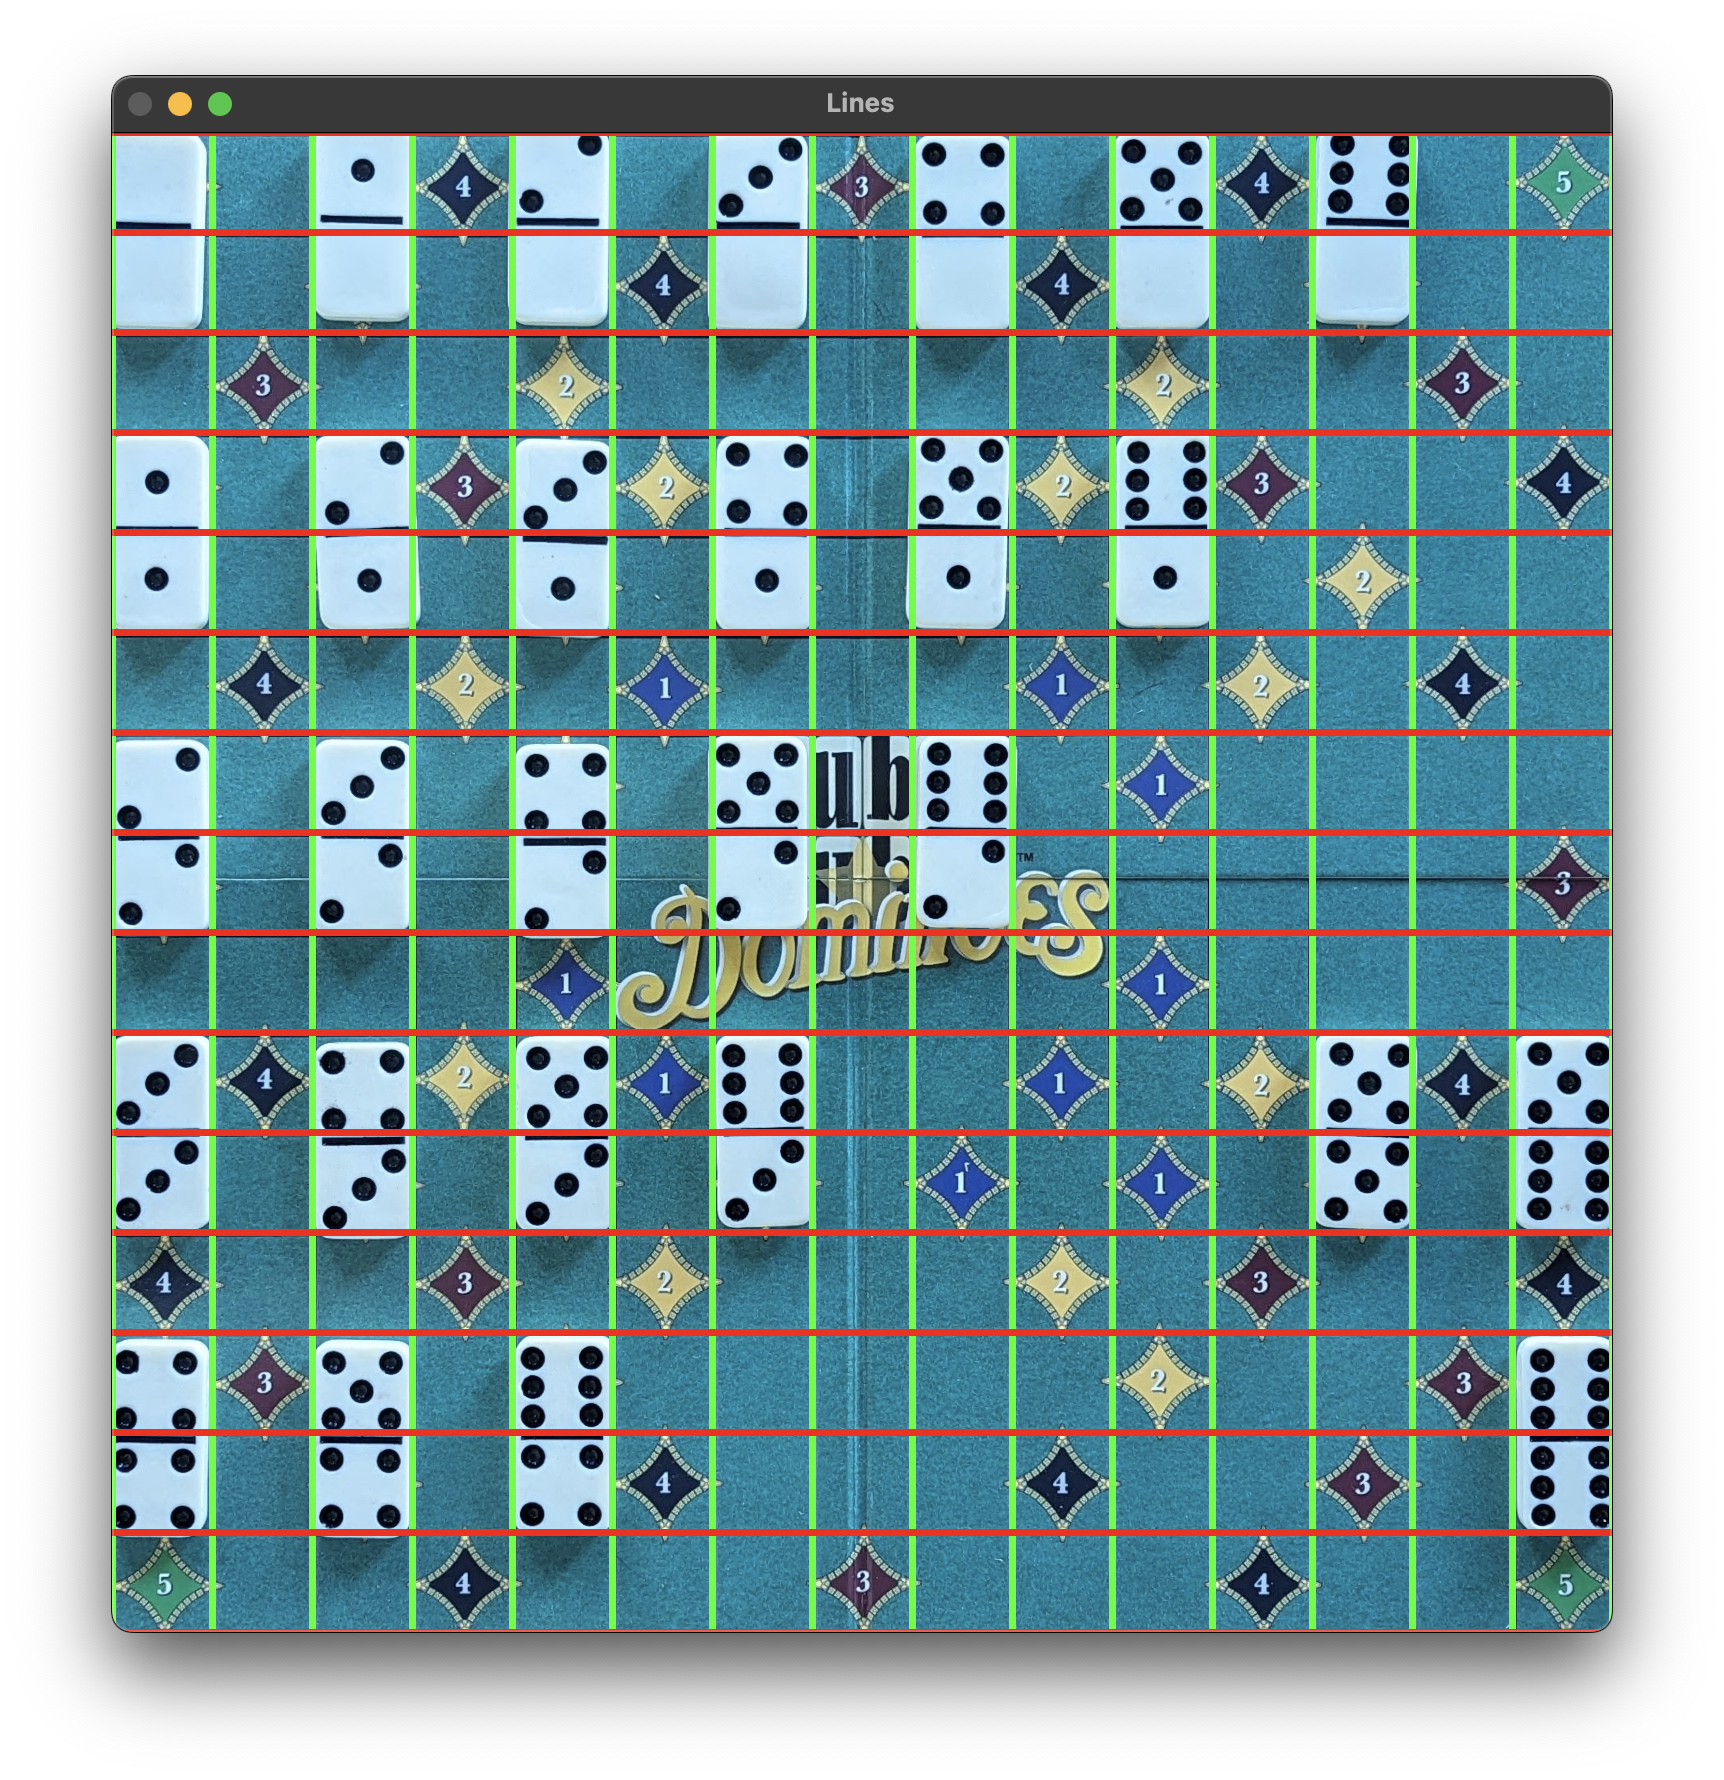
\includegraphics[width=0.9\linewidth]
            {images/board_extraction/lines.png}
            \caption{Lines}
            \label{fig:be-lines}
        \end{subfigure}
    \end{figure}

    \subsection{Piece Detection}\label{subsec:piece-detection}

    \begin{itemize}
        \item The core idea is to use the same mask as before and get each patch at a time, calculate the mean value of the pixels and use a threshold to detect if there is a piece of domino or not.
        \item We've faced two main problems here, the center of the board appears in the mask, (the text of Double Double Dominoes is white therefore appears in the mask) and some pieces are not placed correctly, therefore the black pixels from the board appear in the image influencing the mean.
        \item The center text problem is solved by using template matching. I've created templates from the auxiliary images with each patch of the center text, and if they match we ignore that when detecting. The created templates can be visualized in \hyperref[fig:center-text-template-creation]{Figure 3}.
        \begin{figure}[!h]
            \centering
            \label{fig:center-text-template-creation}
            \begin{subfigure}{.5\textwidth}
                \centering
                \includegraphics[width=0.9\linewidth]{images/center_text_templates/1.png}
                \caption{Center Text Template Example 1}
                \label{fig:ctt-1}
            \end{subfigure}%
            \begin{subfigure}{.5\textwidth}
                \centering
                \includegraphics[width=0.9\linewidth]
                {images/center_text_templates/2.png}
                \caption{Center Text Template Example 2}
                \label{fig:ctt-2}
            \end{subfigure}
            \caption{Center Text Template Creation}
        \end{figure}
        \item The bad placed dominoes problem I've solved by not using the entire patch, but removing 15 pixels from each side, remaining with a 70x70px patch.
        \item The way we create the mask and use it in our algorithm to calculate mean and detect pieces can be visualized in \hyperref[fig:detection]{Figure 4}
        \begin{figure}[!h]
            \centering
            \label{fig:detection}
            \begin{subfigure}{.5\textwidth}
                \centering
                \includegraphics[width=0.9\linewidth]{images/detection/mask1.png}
                \caption{Piece Detection Mask 1}
                \label{fig:pdm-2}
            \end{subfigure}%
            \begin{subfigure}{.5\textwidth}
                \centering
                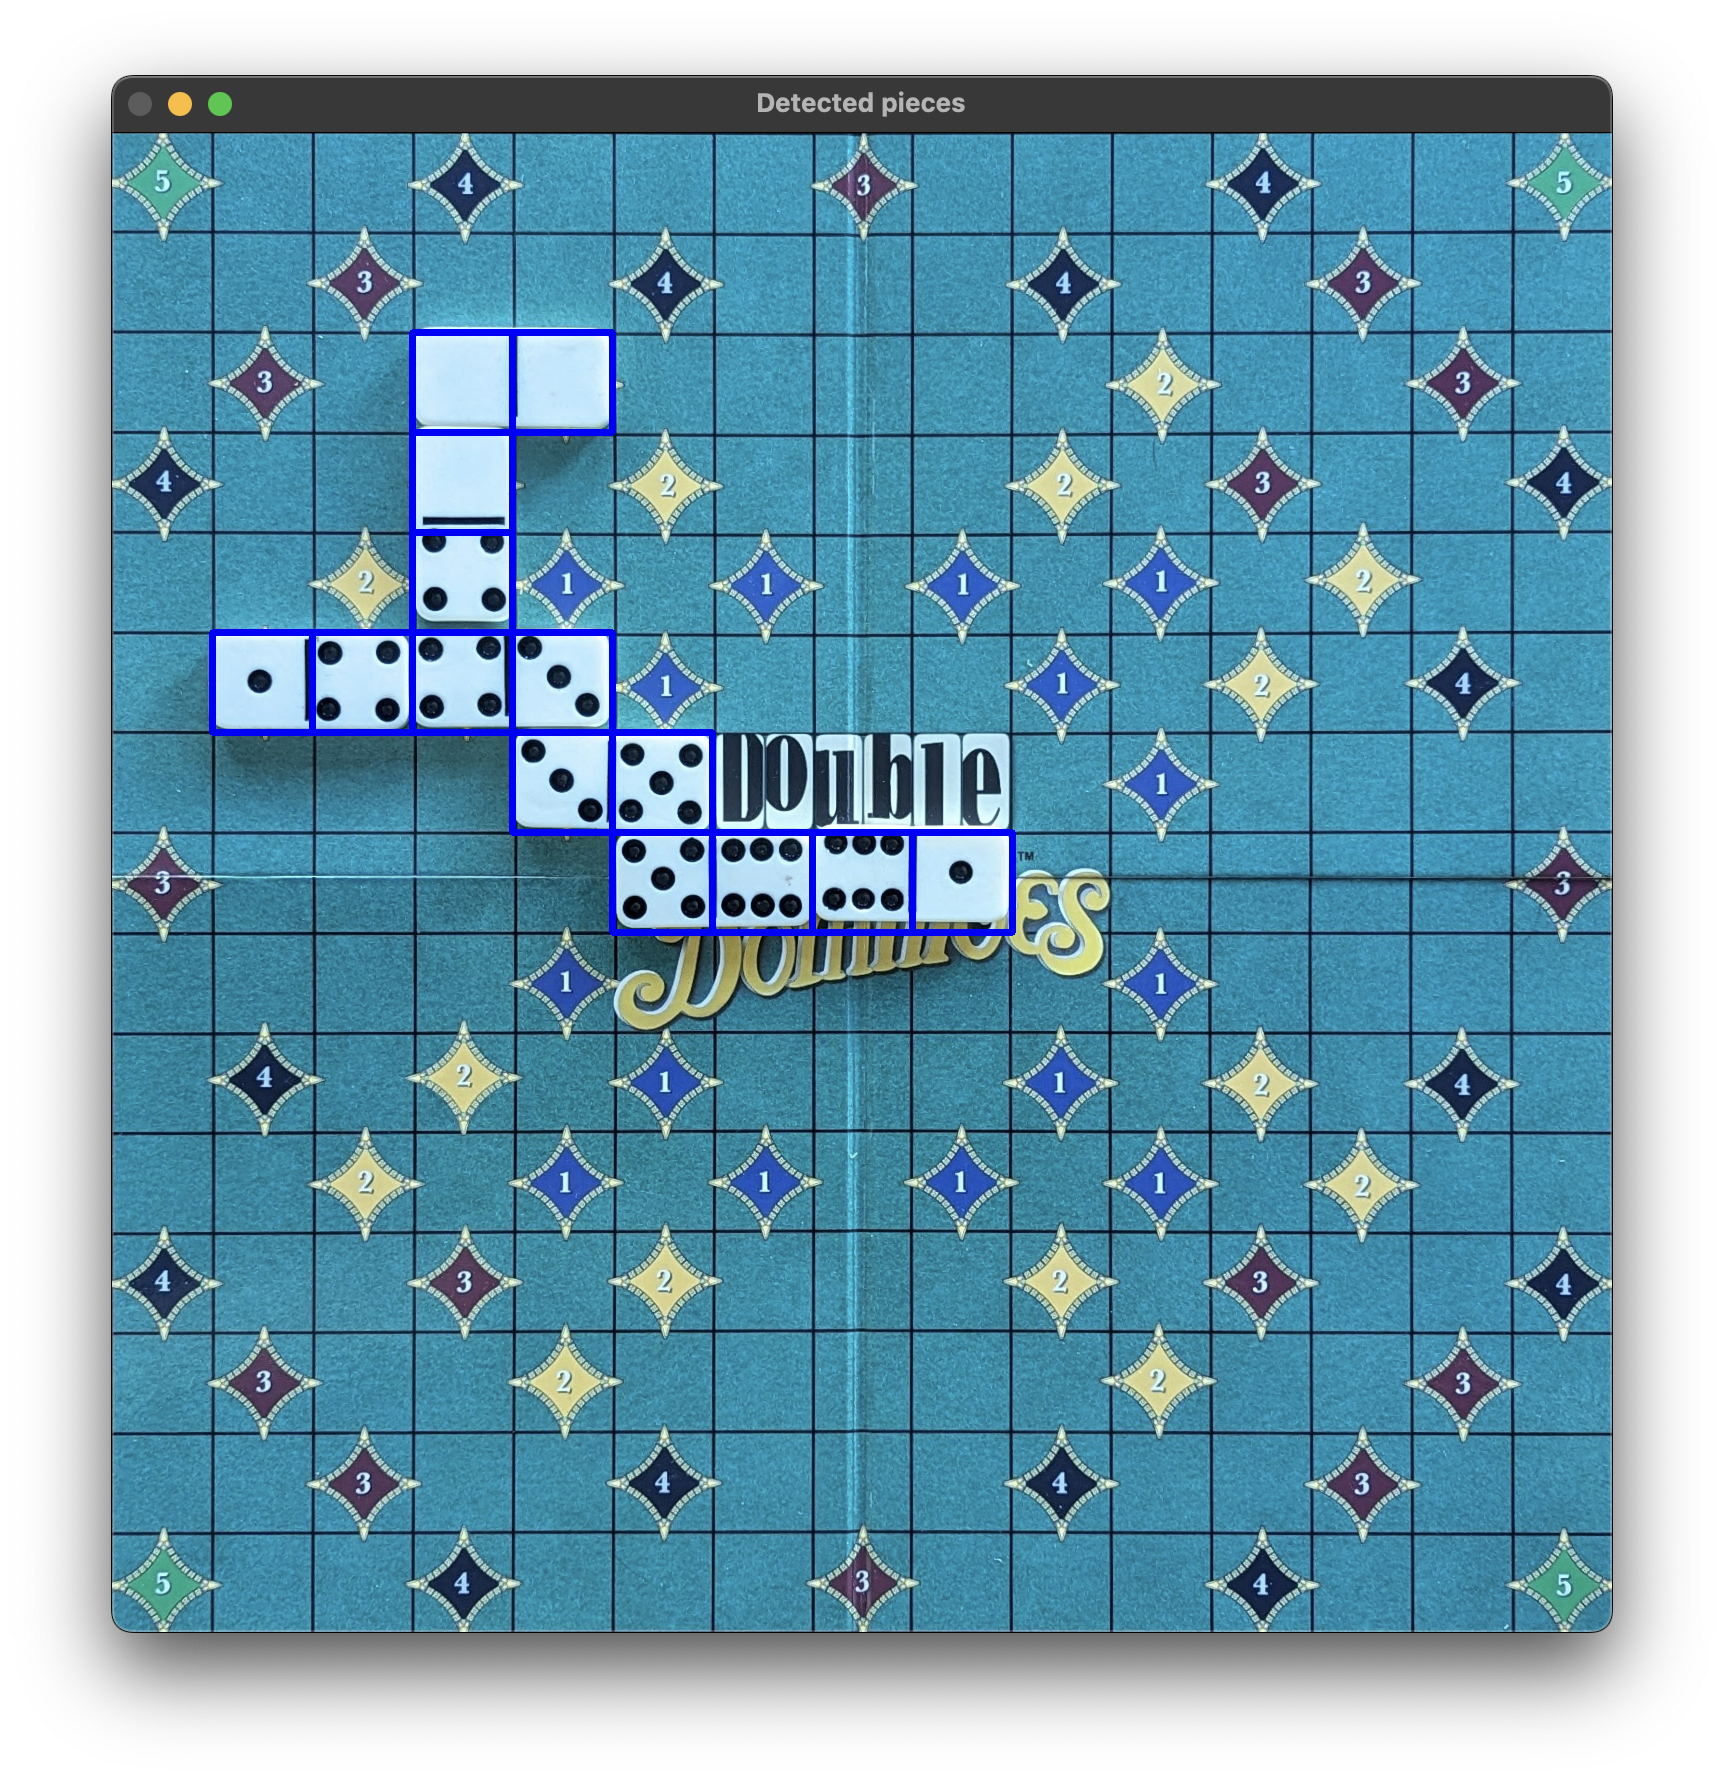
\includegraphics[width=0.9\linewidth]
                {images/detection/detection1.png}
                \caption{Piece Detection Visualization 1}
                \label{fig:pdv-1}
            \end{subfigure}
        \end{figure}
        \begin{figure}[!h]
            \ContinuedFloat
            \centering
            \begin{subfigure}{.5\textwidth}
                \centering
                \includegraphics[width=0.9\linewidth]{images/detection/mask2.png}
                \caption{Piece Detection Mask 2}
                \label{fig:pdm-2}
            \end{subfigure}%
            \begin{subfigure}{.5\textwidth}
                \centering
                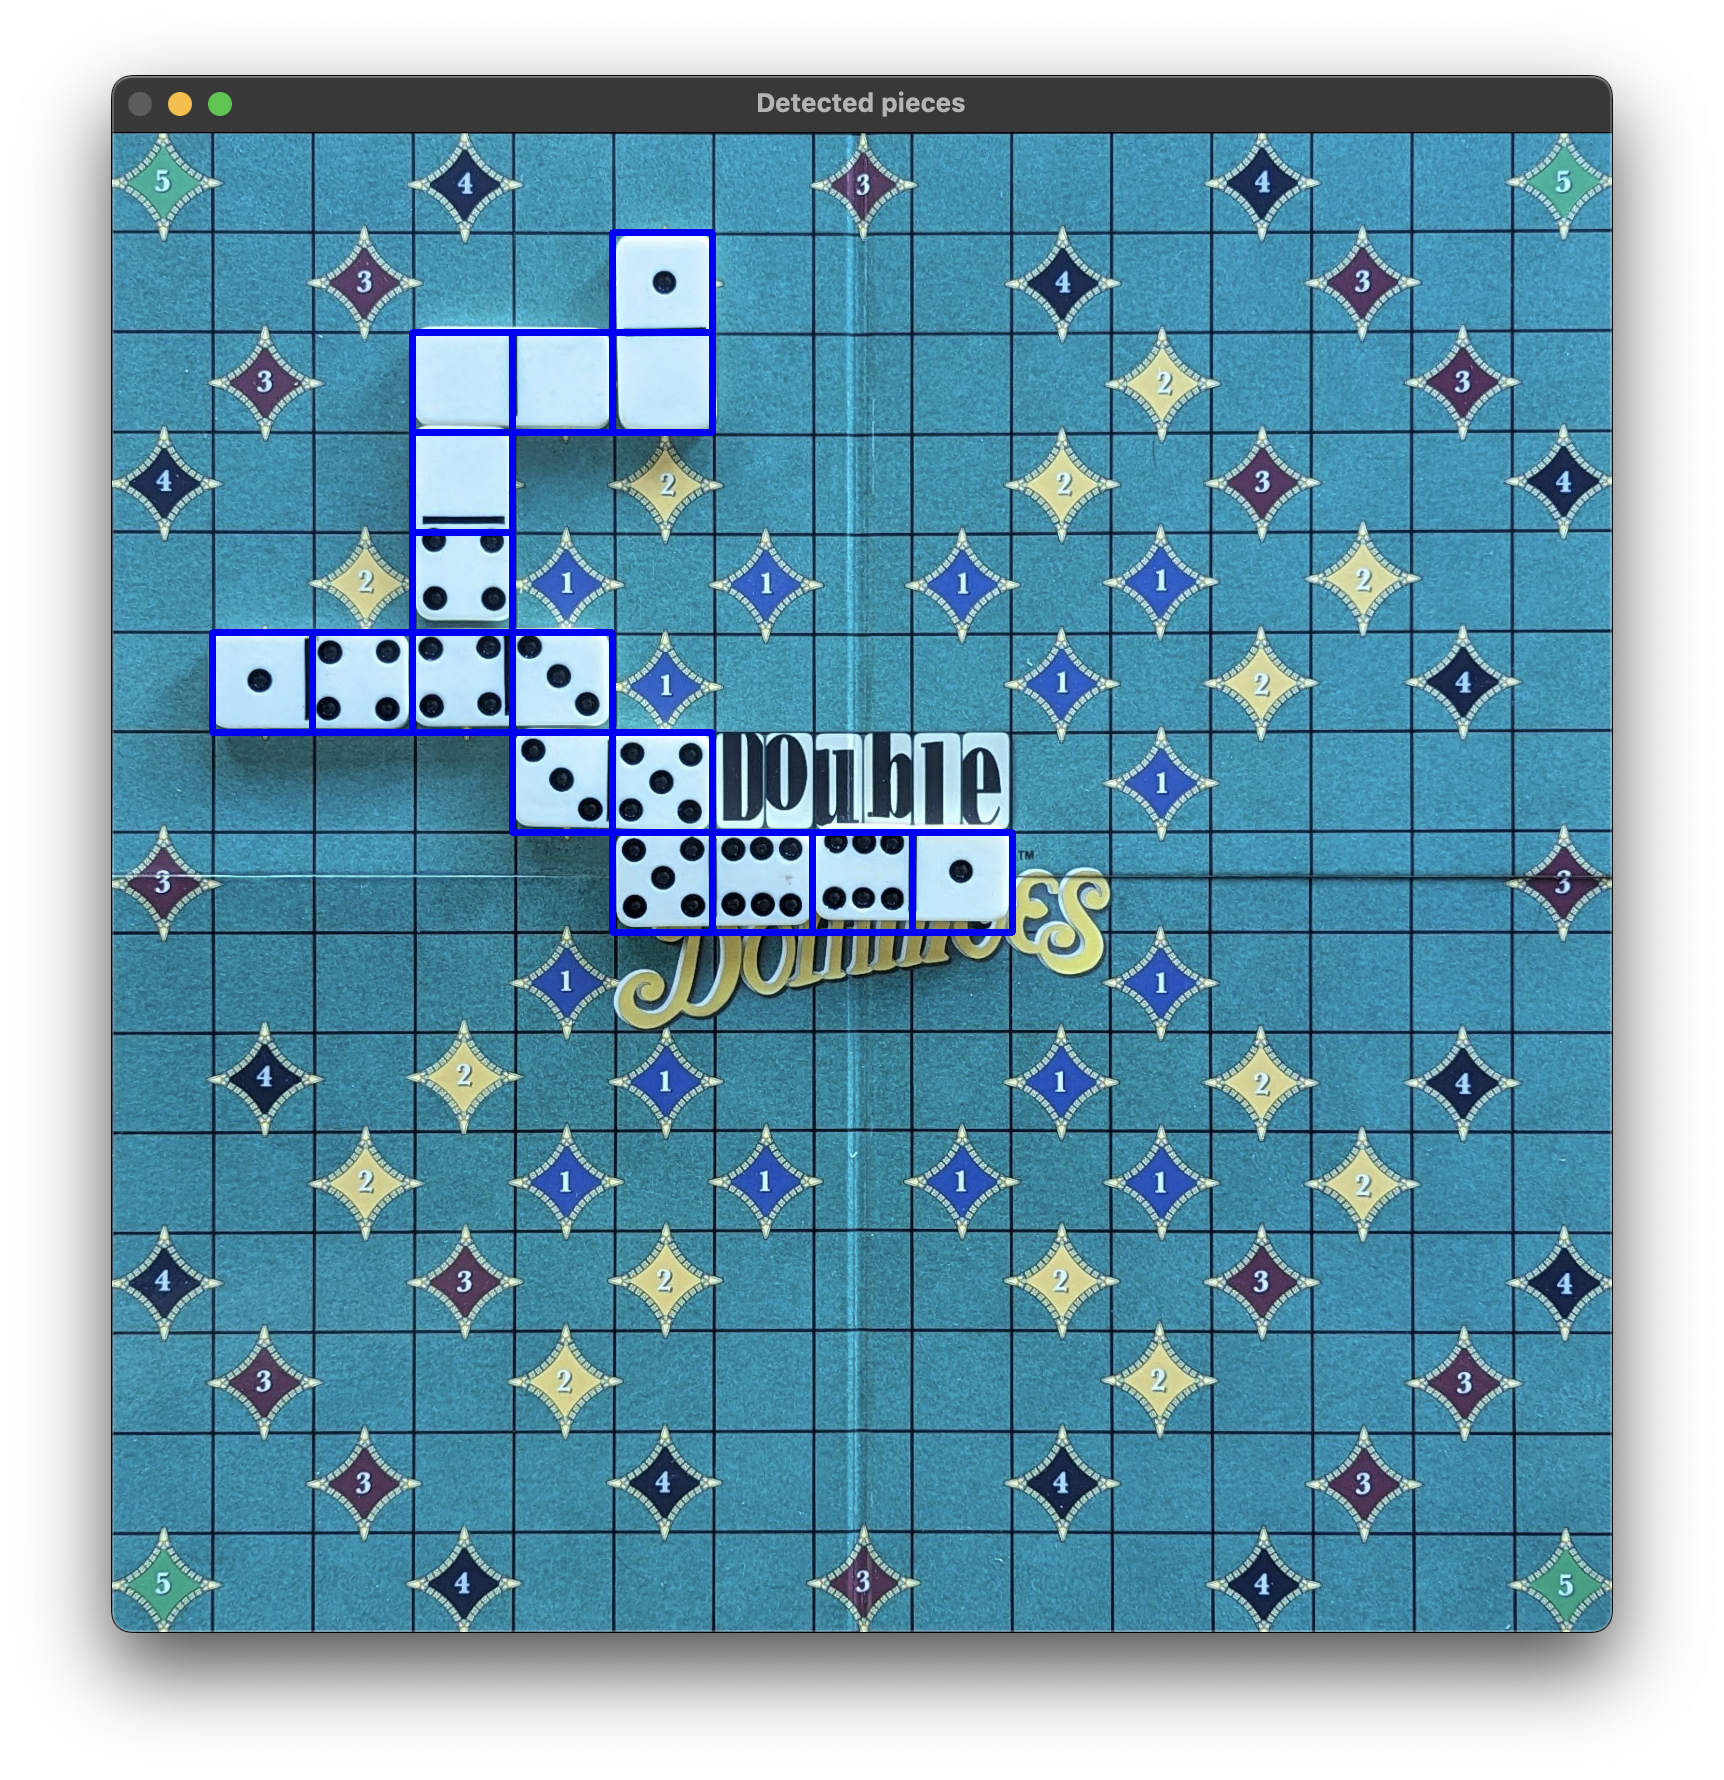
\includegraphics[width=0.9\linewidth]
                {images/detection/detection2.png}
                \caption{Piece Detection Visualization 2}
                \label{fig:pdv-2}
            \end{subfigure}
            \caption{Piece Detection Steps}
        \end{figure}
    \end{itemize}


    \section{Classification}\label{sec:classification}

    \subsection{Templates Creation}\label{subsec:templates-creation}

    \paragraph{For template creation I used a programatic approach, to remove human error. I hardcoded the places on both the vertical and horizontal auxiliary images.}

    \paragraph{Using the board extraction function explained in section \ref{subsec:board-extraction}. I parse the board and whenever I find a place of interest, I know the patch true value, and add it in a list corresponding to its value. (I create templates for both vertical and horizontal placed pieces since domino piece number 3 for example is different depending on the direction it is placed).}

    \paragraph{After saving multiple templates for each domino piece both vertically, and horizontally, I generate the mean image for each direction and value, and save them in a folder for future use.}

    \paragraph{Some examples of the generated templates can be visualized in \hyperref[fig:templates-creation]{Figure 5}.}

    \begin{figure}[!h]
        \centering
        \caption{Templates Creation}
        \label{fig:templates-creation}
        \begin{subfigure}{.5\textwidth}
            \centering
            \includegraphics[width=0.9\linewidth]{images/templates_no_preprocess/horizontal/3.png}
            \caption{Horizontal 3}
            \label{fig:tc-h3}
        \end{subfigure}%
        \begin{subfigure}{.5\textwidth}
            \centering
            \includegraphics[width=0.9\linewidth]
            {images/templates_no_preprocess/vertical/3.png}
            \caption{Vertical 3}
            \label{fig:tc-v3}
        \end{subfigure}
    \end{figure}
    \begin{figure}[!h]
        \ContinuedFloat
        \centering
        \begin{subfigure}{.5\textwidth}
            \centering
            \includegraphics[width=0.9\linewidth]{images/templates_no_preprocess/horizontal/6.png}
            \caption{Horizontal 6}
            \label{fig:tc-h6}
        \end{subfigure}%
        \begin{subfigure}{.5\textwidth}
            \centering
            \includegraphics[width=0.9\linewidth]
            {images/templates_no_preprocess/vertical/6.png}
            \caption{Vertical 6}
            \label{fig:tc-v6}
        \end{subfigure}
    \end{figure}

    \subsection{Template Matching}\label{subsec:template-matching}

    \paragraph{For template matching we use the matchTemplate function from opencv with TM\_COEFF\_NORMED.}

    \paragraph{The main trick for good results is to preprocess the patches. We remove noise, try to remove the lines and board from bad placed pieces, also preprocess the templates, and then call the template matching function.}

    \paragraph{For preprocessing we once again use morphological operations.}
    \begin{lstlisting}[language=Python]
    kernel = np.ones((3, 3), np.uint8)
    image = cv.dilate(image, kernel, iterations=4)
    image = cv.erode(image, kernel, iterations=5)
    \end{lstlisting}

    \paragraph{The preprocess result on extracted patches from the table can be visualized in \hyperref[fig:patch-preprocessing]{Figure 7}, and the templates preprocessing result is also represented in \hyperref[fig:templates-preprocessing]{Figure 6}}

    \begin{figure}[!h]
        \centering
        \label{fig:templates-preprocessing}
        \begin{subfigure}{.5\textwidth}
            \centering
            \includegraphics[width=0.9\linewidth]{images/templates_no_preprocess/vertical/3.png}
            \caption{Original Template 1}
            \label{fig:ot-1}
        \end{subfigure}%
        \begin{subfigure}{.5\textwidth}
            \centering
            \includegraphics[width=0.9\linewidth]
            {images/templates_preprocess/vertical/3.png}
            \caption{Preprocessed Template 1}
            \label{fig:pt-1}
        \end{subfigure}
    \end{figure}
    \begin{figure}[!h]
        \ContinuedFloat
        \centering
        \begin{subfigure}{.5\textwidth}
            \centering
            \includegraphics[width=0.9\linewidth]{images/templates_no_preprocess/horizontal/6.png}
            \caption{Original Template 2}
            \label{fig:ot-2}
        \end{subfigure}%
        \begin{subfigure}{.5\textwidth}
            \centering
            \includegraphics[width=0.9\linewidth]
            {images/templates_preprocess/horizontal/6.png}
            \caption{Preprocessed Template 2}
            \label{fig:pt-2}
        \end{subfigure}
        \caption{Preprocessing Templates Visualization}
    \end{figure}

    \begin{figure}[!h]
        \centering
        \label{fig:patch-preprocessing}
        \begin{subfigure}{.5\textwidth}
            \centering
            \includegraphics[width=0.9\linewidth]{images/patch_preprocessing/original1.png}
            \caption{Original Patch 1}
            \label{fig:op-1}
        \end{subfigure}%
        \begin{subfigure}{.5\textwidth}
            \centering
            \includegraphics[width=0.9\linewidth]
            {images/patch_preprocessing/preproc1.png}
            \caption{Preprocessed Patch 1}
            \label{fig:pp-1}
        \end{subfigure}
    \end{figure}
    \begin{figure}[!h]
        \ContinuedFloat
        \centering
        \begin{subfigure}{.5\textwidth}
            \centering
            \includegraphics[width=0.9\linewidth]{images/patch_preprocessing/original2.png}
            \caption{Original Patch 2}
            \label{fig:op-2}
        \end{subfigure}%
        \begin{subfigure}{.5\textwidth}
            \centering
            \includegraphics[width=0.9\linewidth]
            {images/patch_preprocessing/preproc2.png}
            \caption{Preprocessed Patch 2}
            \label{fig:pp-2}
        \end{subfigure}
        \caption{Preprocessing Patches Visualization}
    \end{figure}


    \section{Score Calculation}\label{sec:score-calculation}

    \paragraph{For score calculation, once the detection and classification work well, there is only a simple dynamic programming approach.}

    \paragraph{Since the score is related to the current position of each player on the score board (aka. their total score) we must save that data constantly at each step. On each move we calculate the current score of the player moving the piece by checking the hardcoded bonus values from the tables, by checking if it is a double piece (3,3 / 6,6 etc.) and by checking for both players if the value placed is the same as their current position on the score board.}

\end{document}
